\documentclass[11pt,a4paper]{report}
\usepackage[a4paper, left=20mm, right=20mm, top=30mm, bottom=20mm]{geometry}
\usepackage{amsmath,amsfonts,amssymb,amsthm,caption,epsfig,epstopdf,float, subcaption, tikz, titling,url,array,tkz-berge}
\usepackage[T2A,T1]{fontenc}
\usepackage[utf8]{inputenc}
\usepackage[russian]{babel}
\usepackage{xparse}
\usepackage[shortlabels]{enumitem}
\usepackage[]{algorithm2e}

\usepackage{hyperref}
\hypersetup{
	colorlinks=true,
	linkcolor=blue,
	filecolor=magenta,      
	urlcolor=cyan,
}

\def\E{\mathbb{E}}
\def\Var{\mathrm{Var}}
\def\Cov{\mathrm{cov}}
\def\Corr{\mathrm{corr}}
\def\salg{\mathcal{F}}
\def\prob{\mathbb{P}}
\def\borel{\mathcal{B}}
\def\cantor{\mathcal{C}}

\def\eps{\varepsilon}
\def\phi{\varphi}
\def\Real{\mathbb{R}}
\def\Proj{\mathbb{P}}
\def\Hyper{\mathbb{H}}
\def\Integer{\mathbb{Z}}
\def\Natural{\mathbb{N}}
\def\Complex{\mathbb{C}}
\def\Rational{\mathbb{Q}}

\def\le{\leqslant}
\def\ge{\geqslant}

\usepackage{stackengine,graphicx,amssymb}
\stackMath
\newcommand\frightarrow{\scalebox{1}[.3]{$\rule[.45ex]{2ex}{1.5pt}%
		\kern-.2ex{\blacktriangleright}$}}
\newcommand\darrow[1][]{\mathrel{\stackon[1pt]{\stackanchor[1pt]{\frightarrow}{\frightarrow}}{\scriptstyle#1}}}

\newcommand\independent{\protect\mathpalette{\protect\independenT}{\perp}}
\def\independenT#1#2{\mathrel{\rlap{$#1#2$}\mkern2mu{#1#2}}}
\renewcommand{\thesection}{\arabic{section}}


\theoremstyle{definition}
\newtheorem{task}{Задача}[section]
\newtheorem*{utask}{Задача}

\theoremstyle{definition}
\newtheorem{theorem}{Теорема}[section]
\newtheorem{lemma}{Лемма}[section]
\newtheorem{preposition}{Утверждение}
\newtheorem*{corollary}{Следствие}

\theoremstyle{definition}
\newtheorem*{definition}{Определение}
\newtheorem{example}{Пример}[section]

\newcommand\mydots{\makebox[1em][c]{.\hfil.\hfil.}}

\title{Совместный анализ QTLs и сетей взаимодействий в дрожжах Saccharomyces cerevisiae}
\author{Вячеслав Иванов, ФИВТ МФТИ\\Научный руководитель: Притыкин Юрий Львович}

\makeatletter
\renewenvironment{thebibliography}[1]
{\section{\refname}%
	\@mkboth{\MakeUppercase\refname}{\MakeUppercase\refname}%
	\list{\@biblabel{\@arabic\c@enumiv}}%
	{\settowidth\labelwidth{\@biblabel{#1}}%
		\leftmargin\labelwidth
		\advance\leftmargin\labelsep
		\@openbib@code
		\usecounter{enumiv}%
		\let\p@enumiv\@empty
		\renewcommand\theenumiv{\@arabic\c@enumiv}}%
	\sloppy
	\clubpenalty4000
	\@clubpenalty \clubpenalty
	\widowpenalty4000%
	\sfcode`\.\@m}
{\def\@noitemerr
	{\@latex@warning{Empty `thebibliography' environment}}%
	\endlist}
\makeatother

\usepackage{array}
\newcolumntype{L}[1]{>{\raggedright\let\newline\\\arraybackslash\hspace{0pt}}m{#1}}
\newcolumntype{C}[1]{>{\centering\let\newline\\\arraybackslash\hspace{0pt}}m{#1}}
\newcolumntype{R}[1]{>{\raggedleft\let\newline\\\arraybackslash\hspace{0pt}}m{#1}}

\begin{document}
	\setlength{\parindent}{1cm}
	{\let\newpage\relax\maketitle}
	\tableofcontents
	\graphicspath{ {/home/vvi/Science/eQTL_analysis/img/} } 
	\newpage
	\section{Введение}
	В наиболее общем смысле, \textit{QTLs} — \textit{Quantitative Traits Loci} — участки генома, варианты которых статистически значимо влияют на степень выраженности некоторого количественного признака. В данной работе рассматриваются два типа QTLs: \textit{eQTLs} (признак — уровень экспрессии гена) и \textit{pQTLs} (признак — уровень трансляции мРНК).\\
	
	Выявление QTLs  — один из методов исследования взаимосвязи между генотипом и фенотипом. Анализ экспрессии белков требует проведения сложных и дорогостоящих экспериментов и плохо масштабируется, а получаемые данные часто очень зашумлены. Анализ экспрессии мРНК, напротив, сравнительно дёшев и опирается на отработанные техники, которые позволяют одновременно анализировать экспрессию тысяч генов — ДНК-микрочипы (DNA microarrays), секвенирование РНК (RNA-sequencing) и другие. Такое положение дел объясняет, почему про pQTLs известно гораздо меньше, несмотря на то, что они ближе к медицинским приложениям данной теории. Современные исследования eQTLs проводят на уровне всего генома, в ходе т.н. \textit{genome-wide association studies} — GWAS — полногеномного поиска ассоциаций. Данная работа является примером такого подхода. При анализе человеческих клеток обычно ищут взаимосвязь между однонуклеотидными полиморфизмами (single-nuncleotide polymorphism (SNP)) и заболеваниями человека.\\
	
	eQTLs — горячая тема в современной генетике: в крупнейших научных журналах наподобие Nature, Science и Cell регулярно выходят статьи о генной регуляции экспрессии, по её изучению учреждаются международные консорциумы и проводятся масштабные эксперименты, задействующие от тысяч (люди) до миллионов (дрожжи) исследуемых особей (так называемые когорты). Хорошим примером служит  \href{https://www.nature.com/articles/s41598-018-24219-z}{серия статей}, опубликованных в 2017 году в Nature консорциумом GTEx — The Genotype-Tissue Expression Project. По результатам более чем десятилетних исследований ими была накоплена крупнейшая база данных по экспрессии генов в основных тканях человека, источником которых послужило более 1000 людей, завещавших свои тела науке. Необходимость таких исследований мотивирована тем, что картина экспрессии генов не просто разнится от ткани к ткани, а ещё и зависит от условий среды, в которой находится клетка, что ярко проявляется при исследовании, к примеру, иммунных или раковых клеток. Динамическая природа экспрессии генов, огромные размеры геномов, требующих для анализа суперкомпьютерных мощностей, сложность сети взаимодействий между генами — краткий перечень причин, на основании которых можно утверждать, что в науке об eQTLs (и QTLs в целом) остаётся немало открытых вопросов, имеющих равно как теоретическое, так и прикладное значение.\\
	
	В данной работе рассматривается проблема взаимосвязи eQTLs и pQTLs и подход к её исследованию, основанный на анализе сети белок-белковых взаимодействий. На примере модельного организма — \textit{Saccharomyces cerevisiae} — проверяется гипотеза о связи eQTLs и pQTLs на уровне функциональных модулей — наборов белков, связанных с конкретным клеточным процессом. В перспективе планируется ввести понятие "module QTLs" — QTLs, в некотором смысле управляющих экспрессией функционального модуля как целого. Есть основания полагать, что оно биологически содержательно и представляет научный интерес, но все необходимые определения пока только предстоит чётко сформулировать.\\
	
	Говоря конкретно, исследуемый вопрос формулируется так: почему для подавляющего большинства генов нет видимой взаимосвязи между множествами eQTLs и pQTLs, с ними связанных? В современной науке он остаётся открытым. Противоречие с интуицией, которая утверждает, что связанные процессы должны иметь общие механизмы регуляции, наводит на мысль, что уровни экспрессии генов в мРНК и в белок могут быть связаны на уровне клеточных процессов, а не на уровне индивидуальных молекул. Отсюда возникает идея рассматривать экспрессию в контексте взаимодействий и функций, которые белки выполняют в клетке. Гипотезу о том, что на уровне функциональных модулей между множествами eQTLs и pQTLs есть статистически значимая связь, предлагается проверять с помощью сети белок-белковых взаимодействий. Несмотря на то, что сети взаимодействий нередко критикуют за невоспроизводимость результатов (и правда, структура сети не инвариантна относительно состояния клетки и условий среды, что не улавливается в должной мере существующими базами данных — такими как \href{https://thebiogrid.org/}{The BioGRID}, \href{https://reactome.org/}{Reactome}, \href{http://www.genome.jp/kegg/}{KEGG} и др.), их часто используют, т.к. они наглядны, хорошо изучены и захватывают существенную часть генома Saccharomyces cerevisiae. Для обеспечения же надёжности выводов, полученных с помощью сетей, на каждом шаге исследования принято проверять, что полученные результаты объясняются биологическим смыслом соответствующих подграфов сети, а не их структурными особенностями в отрыве от содержания.
	
	\section{Цели:}
	\begin{enumerate}
		\item Определить множества QTLs для всех генов, для которых измерена экспрессия, контролируя процент ошибок первого рода (должен быть меньше заданного порога). Чтобы гарантировать корректность данных, сравнить получившиеся распределения QTLs в геноме с взятыми из ключевых статей по данной тематике.
		\item Проверить для каждого типа взаимодействий (физические, генетические, их подтипы) гипотезу: множества QTLs взаимодействующих генов пересекаются сильнее, чем у случайно выбранных пар. Более формально еёможно переформулировать так: усреднённая мера подобия множеств QTLs одного типа для взаимодействующих генов выше, чем для случайных пар. Для обеспечения корректности выводов для каждого типа провести рандомизацию её подсети, повторить проверку и сравнить полученные результаты.
		\item Для каждого гена в качестве кандидатов в его pQTLs рассмотреть только eQTLs его соседей, включая его самого. Показать, что при таком подходе и воспроизводится существенная доля результатов, и находятся новые pQTLs. Возможность предсказывать pQTLs на основе eQTLs, если таковая обнаружится, будет аргументом в пользу взаимосвязи между ними.
		\item Для некоторого опубликованного набора функциональных модулей — подграфов сети взаимодействий — оценить среднюю меру подобия множеств QTLs одного типа для взаимодействующих генов и случайных пар, а затем сравнить их. Если гипотеза верна, то зависимость есть, причём в четвёртом пункте она должна быть выражена более ярко, чем во втором.
	\end{enumerate}
	
	\section{Результаты}
	\subsection{Идентификация QTLs}
	   В данной работе исследуются QTLs — участки генома, влияющие на уровень экспрессии генов. Для их определения существуют разные подходы, об этом пишут целые книги (например \href{https://www.springer.com/gp/book/9780387921242}{"A Guide to QTL Mapping with R/qtl", Karl Broman \& Sen Saunak}). Был использован простейший алгоритм, основанный на ранговом тесте Манна-Уитни (Mann-Whitney U, MWU-test). Описание предложенного алгоритма приведено в разделе "Методы".
		\begin{figure}[H]
			\centering
			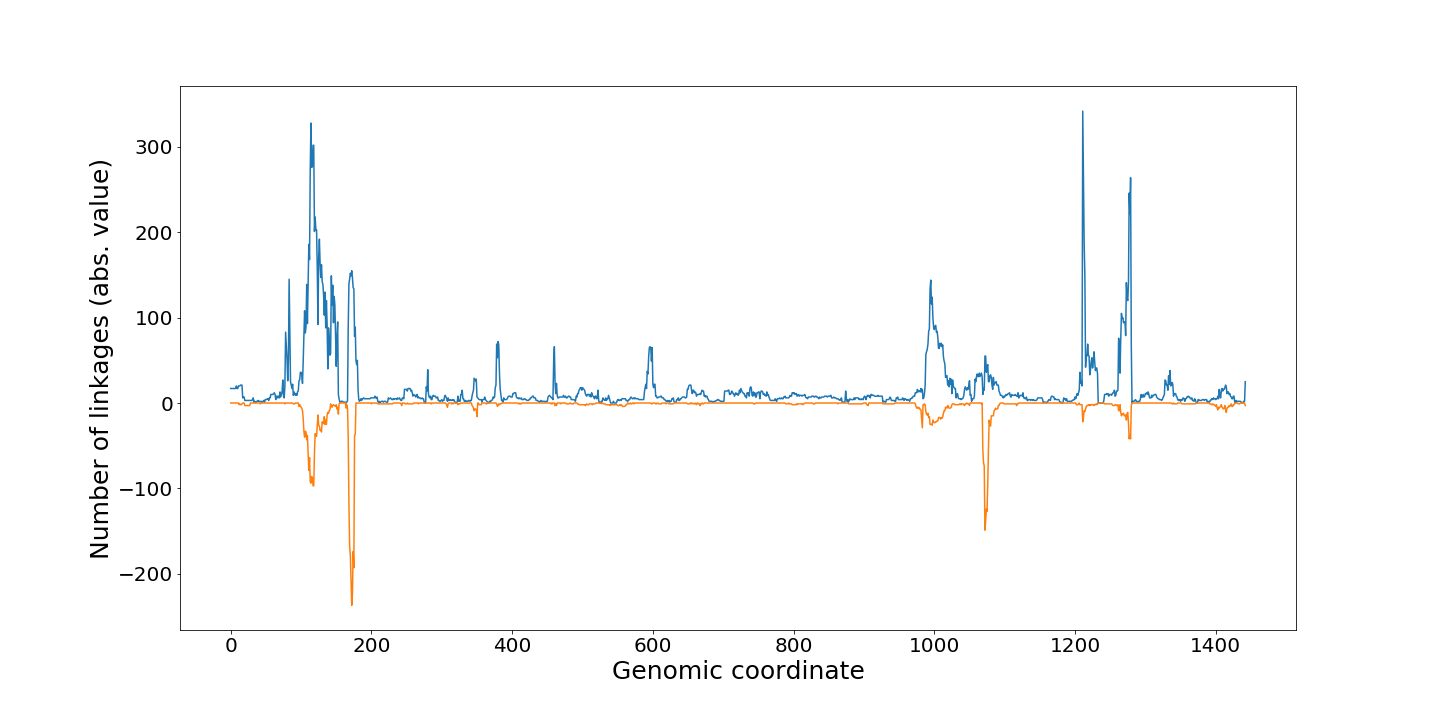
\includegraphics[scale=0.35]{linkages/eQTLs_pQTLs_combined.png}
			\caption{Распределение найденных eQTLs (синий) и pQTLs (оранжевый) в геноме Saccharomyces cerevisiae. По горизонтальной оси отложены позиции маркеров, отсортированных в порядке возрастания геномных координат. Абсолютное значение величины, отложенной на вертикальной оси, отражает число QTLs, связанных с данным участком генома.}
		\end{figure}
		По рисунку 1. видно, что расположение пиков для eQTLs и pQTLs похоже. Наблюдаемые пики в научной литературе называют \textit{hotspots} — участки генома, вариации в которых оказывают существенное влияние на профиль экспрессии генов. Их положение в геноме — видовая черта, устойчивая относительно индивидуальных различий.\\
		
		Для сравнения приведём график из статьи \href{http://science.sciencemag.org/content/296/5568/752.full}{"Genetic Dissection of Transcriptional Regulation in Budding Yeast", 2002}, положившей начало полногеномному eQTL-анализу в дрожжах. Видно, что распределения похожи: расположения основных hotspots совпадают. Разница в распределении высот связана с тем, что использованные данные богаче, чем приведенные в статье.
		
		\begin{figure}[H]
			\centering
			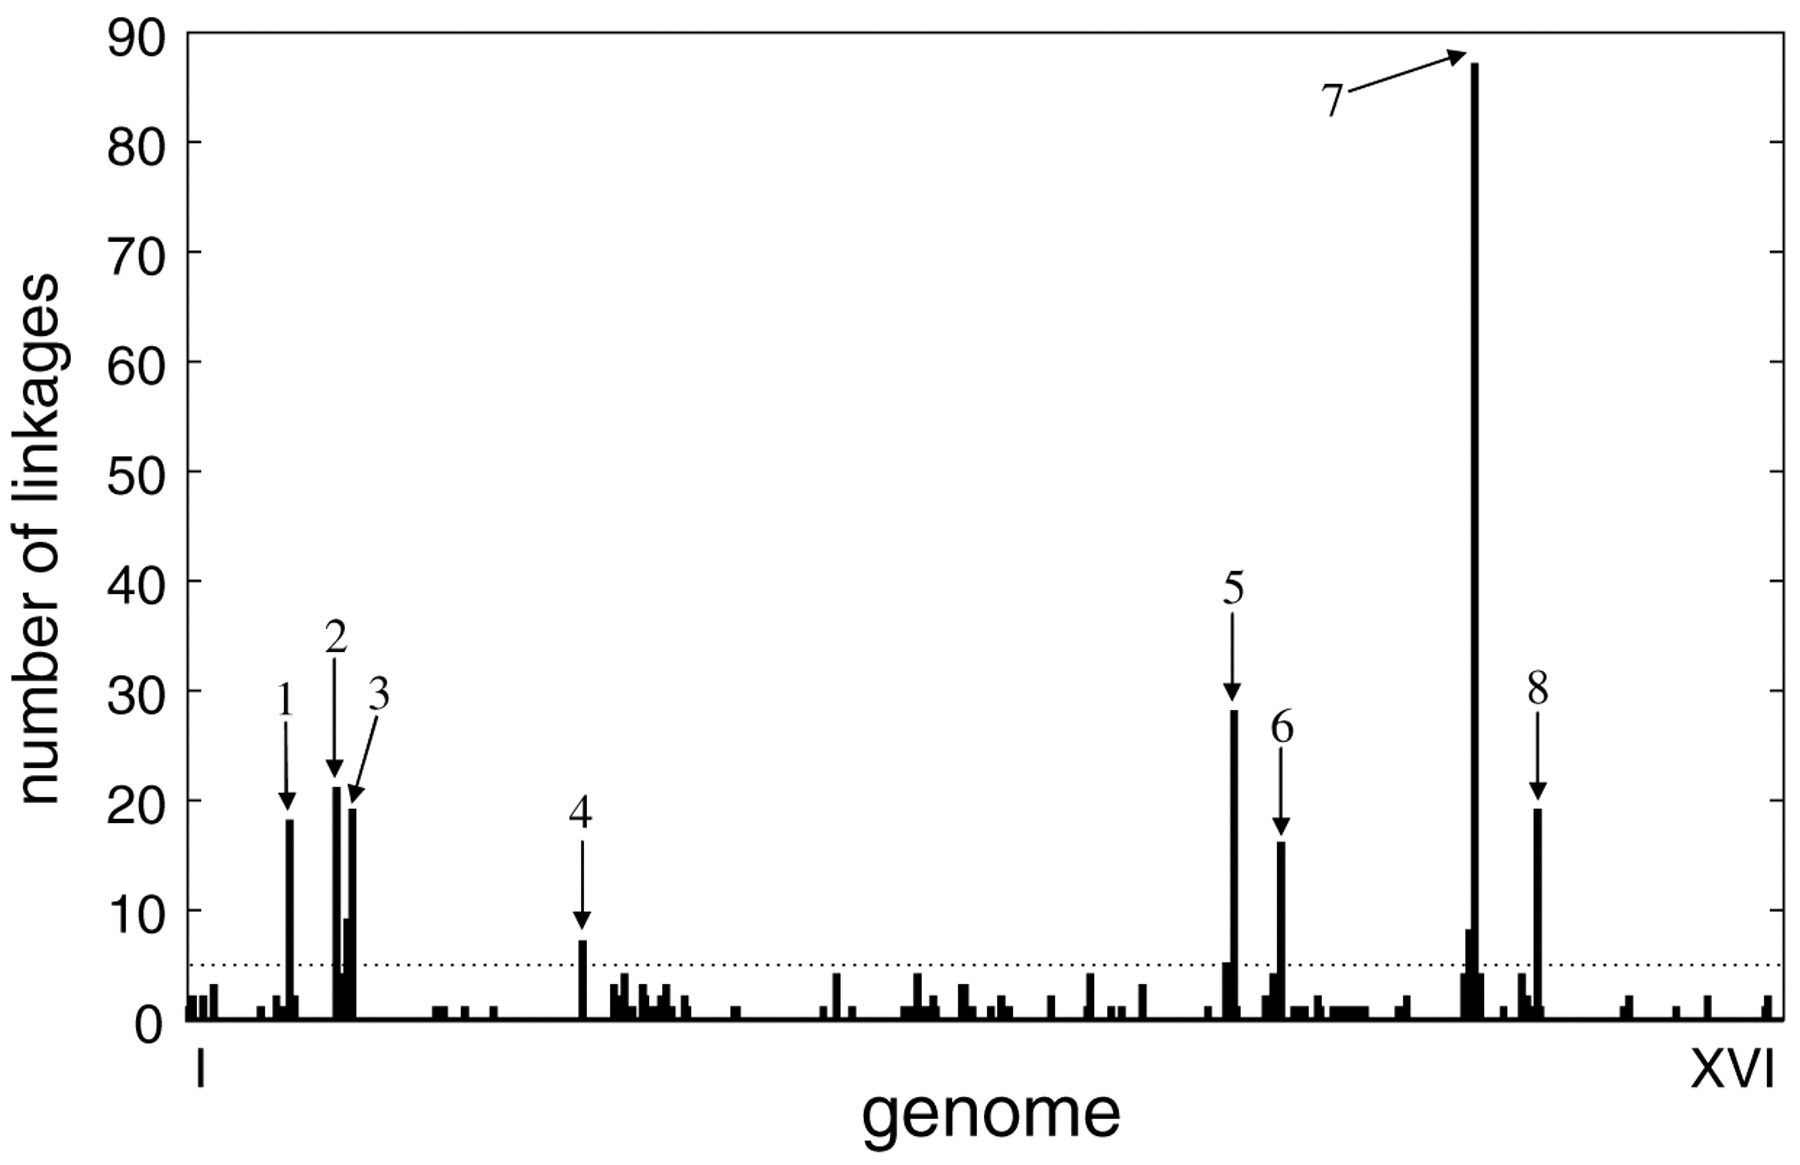
\includegraphics[scale=0.25]{illustrations/Brem_Kruglyak_eQTLs_distribution.jpg}
			\caption{
				Распределение числа eQTLs относительно позиции в геноме. Геном поделен на 611 столбцов шириной в 20 000 оснований в каждом, отсортированных в порядке от начала первой хромосомы до конца шестнадцатой. Штрихованная линия соответствует отсечке в 5 eQTLs: ожидается, что почти наверное ни один из столбцов не будет содержать 5 и больше false positives.\\
				\href{http://science.sciencemag.org/content/296/5568/752.full}{"Genetic Dissection of Transcriptional Regulation in Budding Yeast", doi: 10.1126/science.1069516, 2002} 
		  }
		\end{figure}
		Следовательно, есть основания полагать, что QTLs были определены корректно.
	\subsection{Исследование подобия множеств QTLs у взаимодействующих генов}
		В данной работе исследуется взаимосвязь между eQTLs и pQTLs в контексте взаимодействий между генами. Согласно классификации проекта TheBioGRID, взаимодействия делятся на несколько типов (см. "Методы"). Основной интерес представляет грубая классификация взаимодействий на "генетические" и "физические". Для обеих категорий была подсчитана усреднённая мера подобия множеств QTLs одного типа, связанных с парой взаимодействующих генов — \textit{коэффициент Жаккара} для этих множеств:
		
		\begin{definition}
			Пусть $ A, B $ — конечные множества элементов одного типа (в данном случае — маркеров). Тогда их \textbf{коэффициентом Жаккара} называют величину
			$$ J(A, B) := \left| \frac{|A \cap B|}{|A \cup B|} \right| $$
		\end{definition}
			
	 Затем, для проверки получаемых результатов, была многократно проведена рандомизация подграфа взаимодействий каждого из типов с сохранением некоторых его структурных инвариантов и на каждой итерации была подсчитана аналогичная величина, среднее значение которых также изображено на графиках. Таким образом исключалась возможность того, что наблюдаемая мера подобия есть следствие одной лишь структуры подграфа, без оглядки на его биологический смысл. Конкретный способ рандомизации графа и детали реализации указаны в разделе "Методы". 
		
%		\vspace*{\fill}
%		\begingroup
		\begin{figure}[H]
				\caption{По вертикальной оси отложена усреднённая мера подобия множеств eQTLs, связанных со взаимодействующими генами. В качестве такой меры использовался коэффициент Жаккара. По горизонтальной оси отложены пороги q -значений, по которым определялось подмножество статистически значимых  eQTLs. Синим цветом отрисованы значения, полученные для сети физических взаимодействий, оранжевым цветом — усреднённое по ста итерациям значение в рандомизированной сети. }
				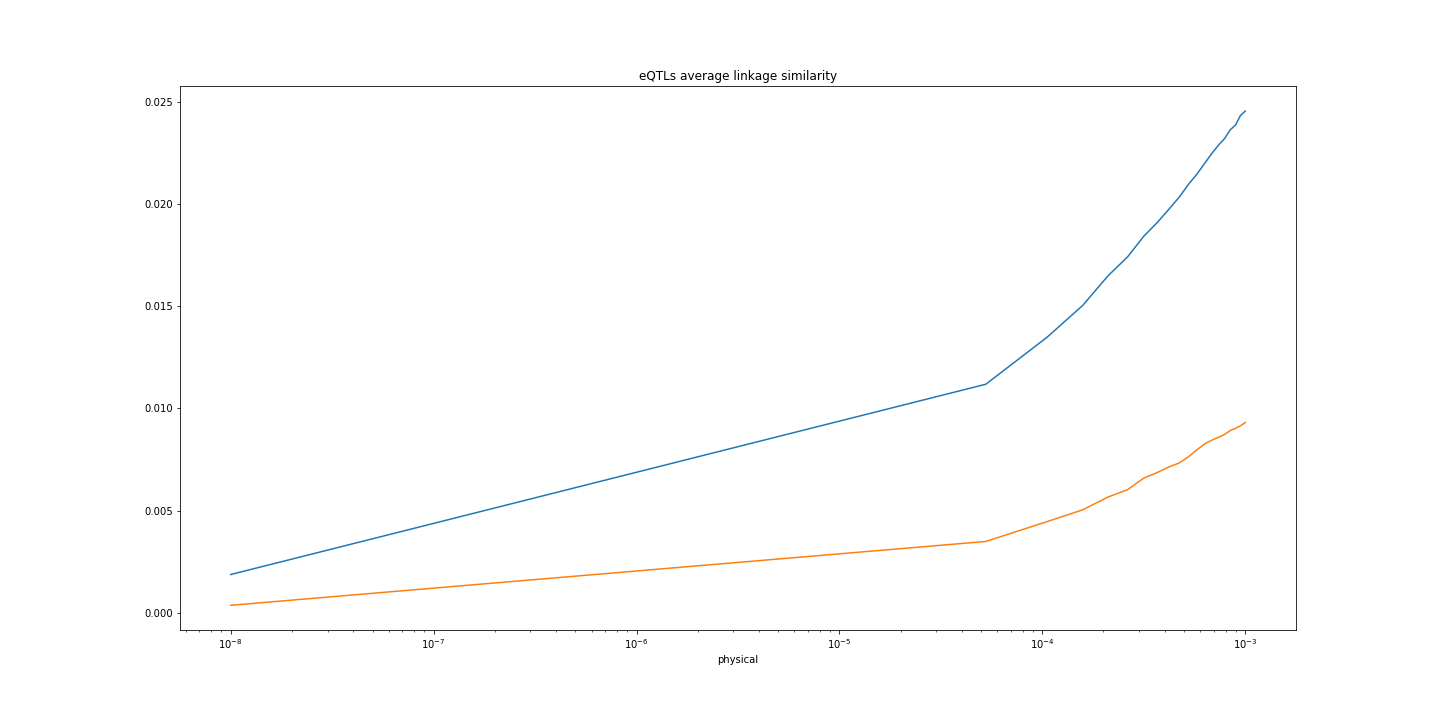
\includegraphics[scale=0.35]{interactions/eQTLs_physical.png}
				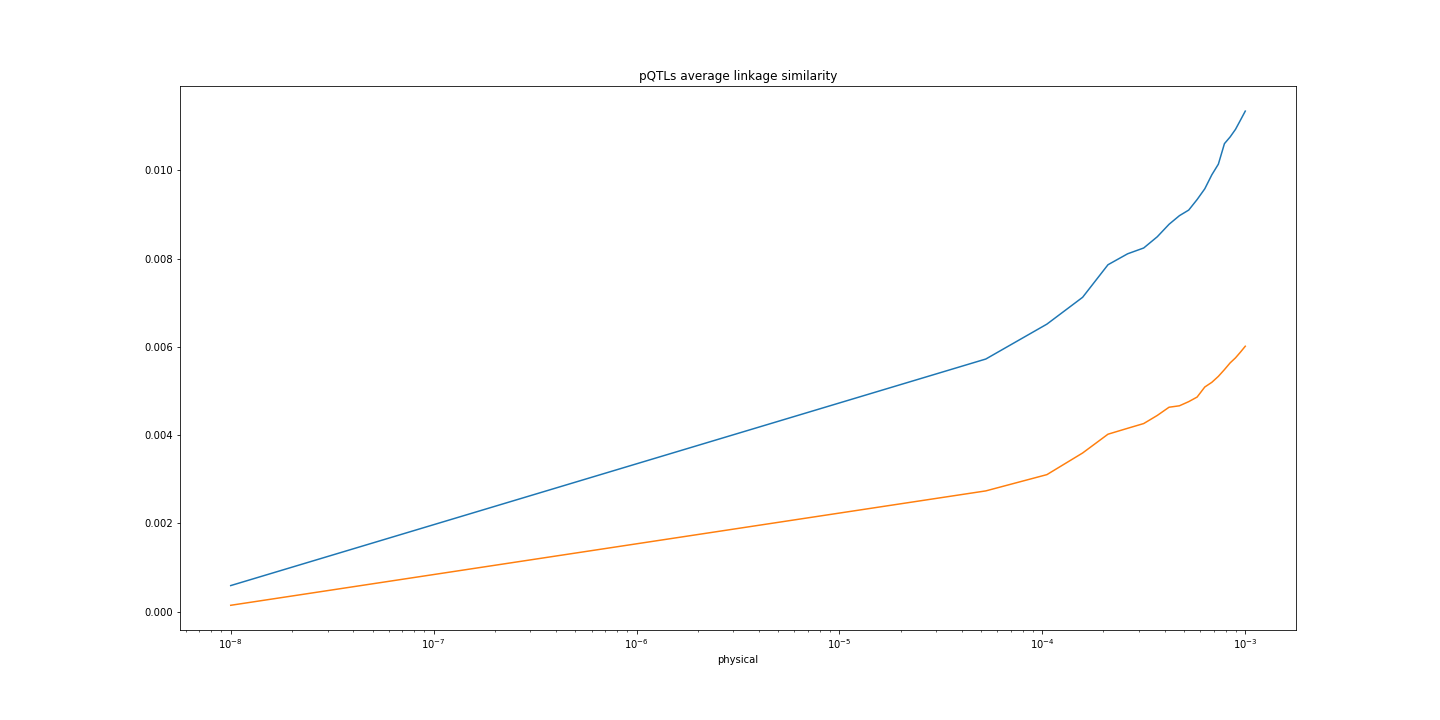
\includegraphics[scale=0.35]{interactions/pQTLs_physical.png}
		\end{figure}
%		\endgroup
%		\vspace*{\fill}
		
		\newpage
		\begin{figure}[H]
			\caption{Аналогично рисунку 3., только теперь для сети генетических взаимодействий.}
			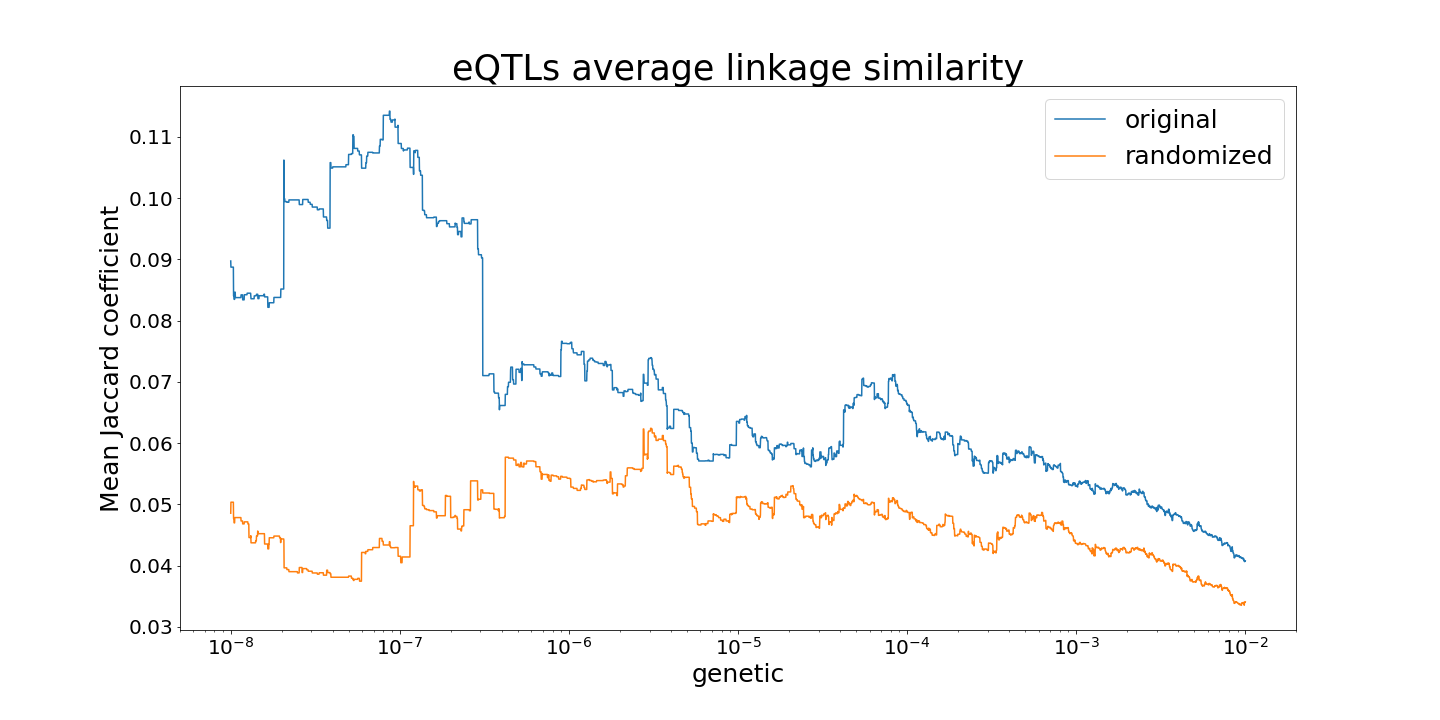
\includegraphics[scale=0.35]{interactions/eQTLs_genetic.png}
			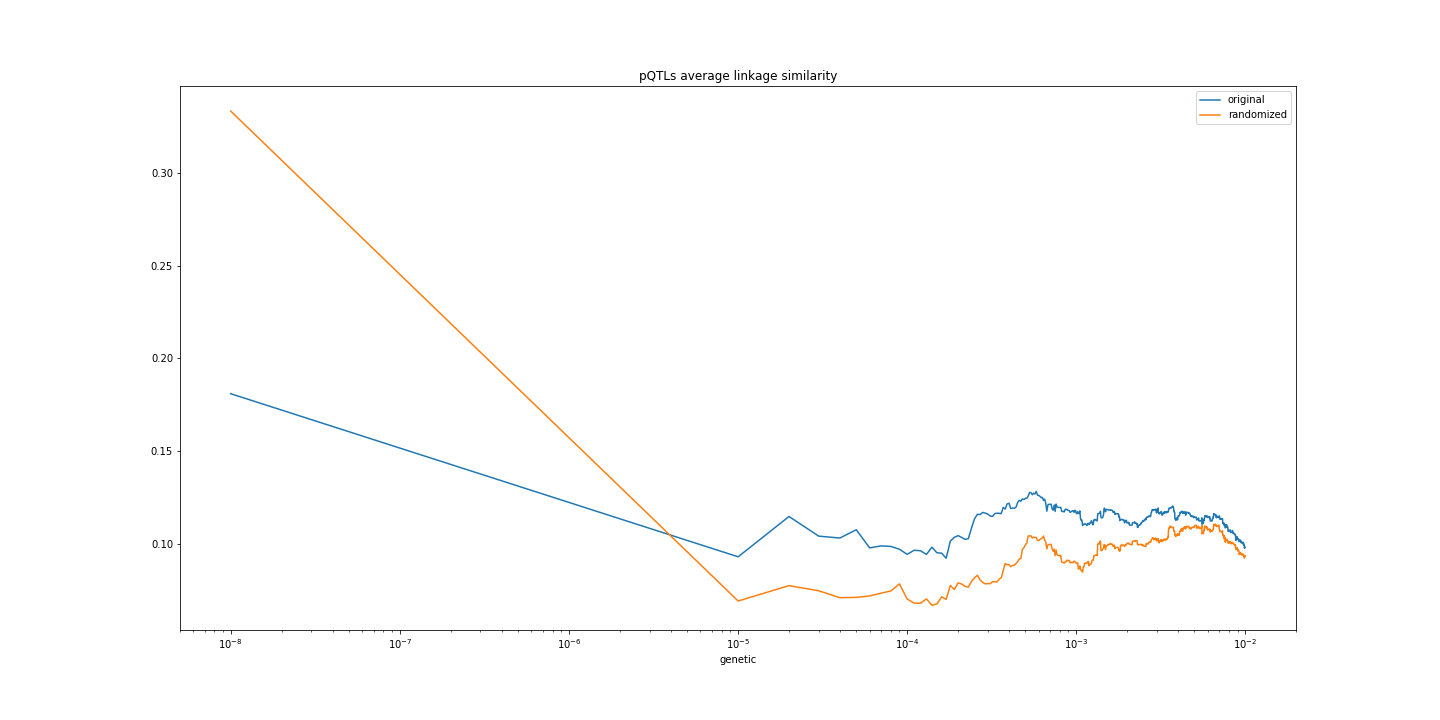
\includegraphics[scale=0.35]{interactions/pQTLs_genetic.png}
		\end{figure}
		
		Компьютерное моделирование подтверждает, что взаимодействующие гены склонны иметь общие QTLs, причём для физических взаимодействий эта зависимость более явная, чем для генетических. Это согласуется с теоретическими представлениями: физические взаимодействия более "непосредственные" и конкретные, часто означают тесную связь между функциями белков.\\
		
		Видно, что менее зашумленные, доступные в б\textbf{о}льших количествах eQTLs лучше иллюстрируют наблюдаемый эффект. Ознакомиться с аналогичными графиками для более тонкой классификации взаимодействий можно \href{https://github.com/ivanov-v-v/eQTL_analysis/tree/master/img/interactions}{по ссылке} (их достаточно много, чтобы не приводить все здесь).\\
	\subsection{Предсказание pQTLs на основе eQTLs}
		Совместное исследование множеств eQTLs и pQTLs показало, что для отдельных генов эти множества пересекаются очень слабо, что иллюстрирует рисунок 5.
		\begin{figure}[H]
			\caption{Для каждого гена, для которого были измерены уровни и экспрессии мРНК, и белковой экспрессии, были рассмотрены множества связанных с ним eQTLs и pQTLs, вычисленных на предыдущем шаге, и для них был подсчитан коэффициент Жаккара. Распределение полученных значений иллюстрирует приведенная гистограмма.}
			\centerline{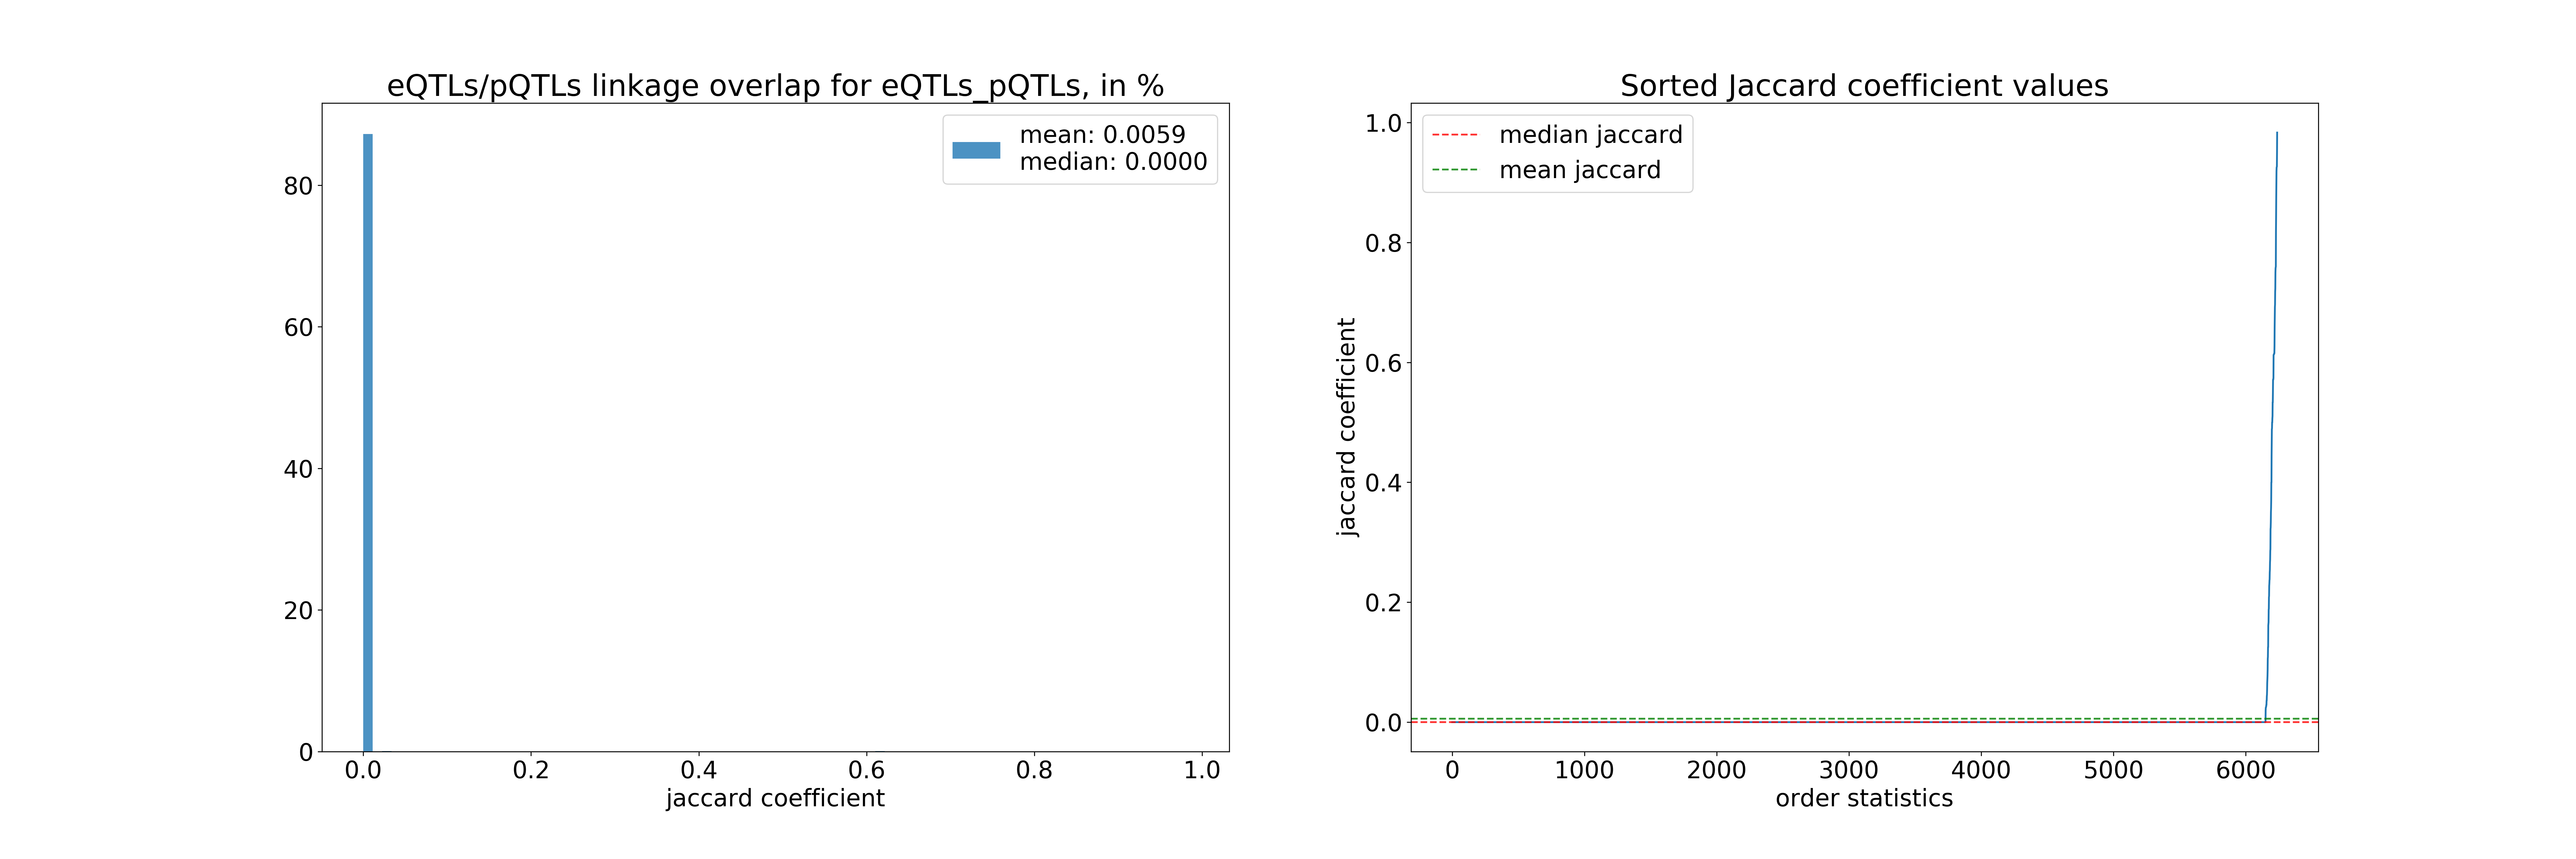
\includegraphics[scale=0.3]{linkages/eQTLs_pQTLs_linkage_overlap.png}}
		\end{figure}
		
		В итоге, кажется, что знание eQTLs, связанных с данным геном, ничего не даёт для предсказания pQTLs для этого гена. Это противоречит интуиции: связанные клеточные процессы, казалось бы, должны иметь общие механизмы регуляции.\\ 
		
		Возникает идея попробовать более тонкие способы поиска взаимосвязей между eQTLs и pQTLs. В частности, была предложена идея в качестве кандидатов в pQTLs для данного гена рассматривать eQTLs его соседей в графе взаимодействий (включая его самого). Сужение кандидатов в pQTLs таким образом при рассмотрении полного графа белок-белковых взаимодействий позволяет найти 6124 pQTLs против 6162 найденных наивным методом (в роли кандидатов в нём выступают все маркеры). Среди них воспроизводится 3695 (~60\%) найденных прежде pQTLs и обнаруживается 2429 (~40\%) новых. Если рассматривать только подграф физических взаимодействий, то находятся 4048 pQTLs, воспроизводятся 2021 (~33\%), соответственно новых среди них 2027 (~50\%). Результаты, полученные применением такого подхода, изображены на рисунке 6.
		\begin{figure}[H]
			\caption{Распределения pQTLs, полученные наивным алгоритмом (синий) и предложенным (оранжевый), запущенным на полном графе взаимодействий. eQTLs были отфильтрованы по пороговому q-значению в 0.05. Видно, что структура положение пиков и распределение их высот воспроизводится. Наблюдаемая разница высот, однако, показывает, что взаимодействия объясняют не могут объяснить все различия в уровнях экспрессии, имеющиеся в экспериментальных данных. } 
			\centerline{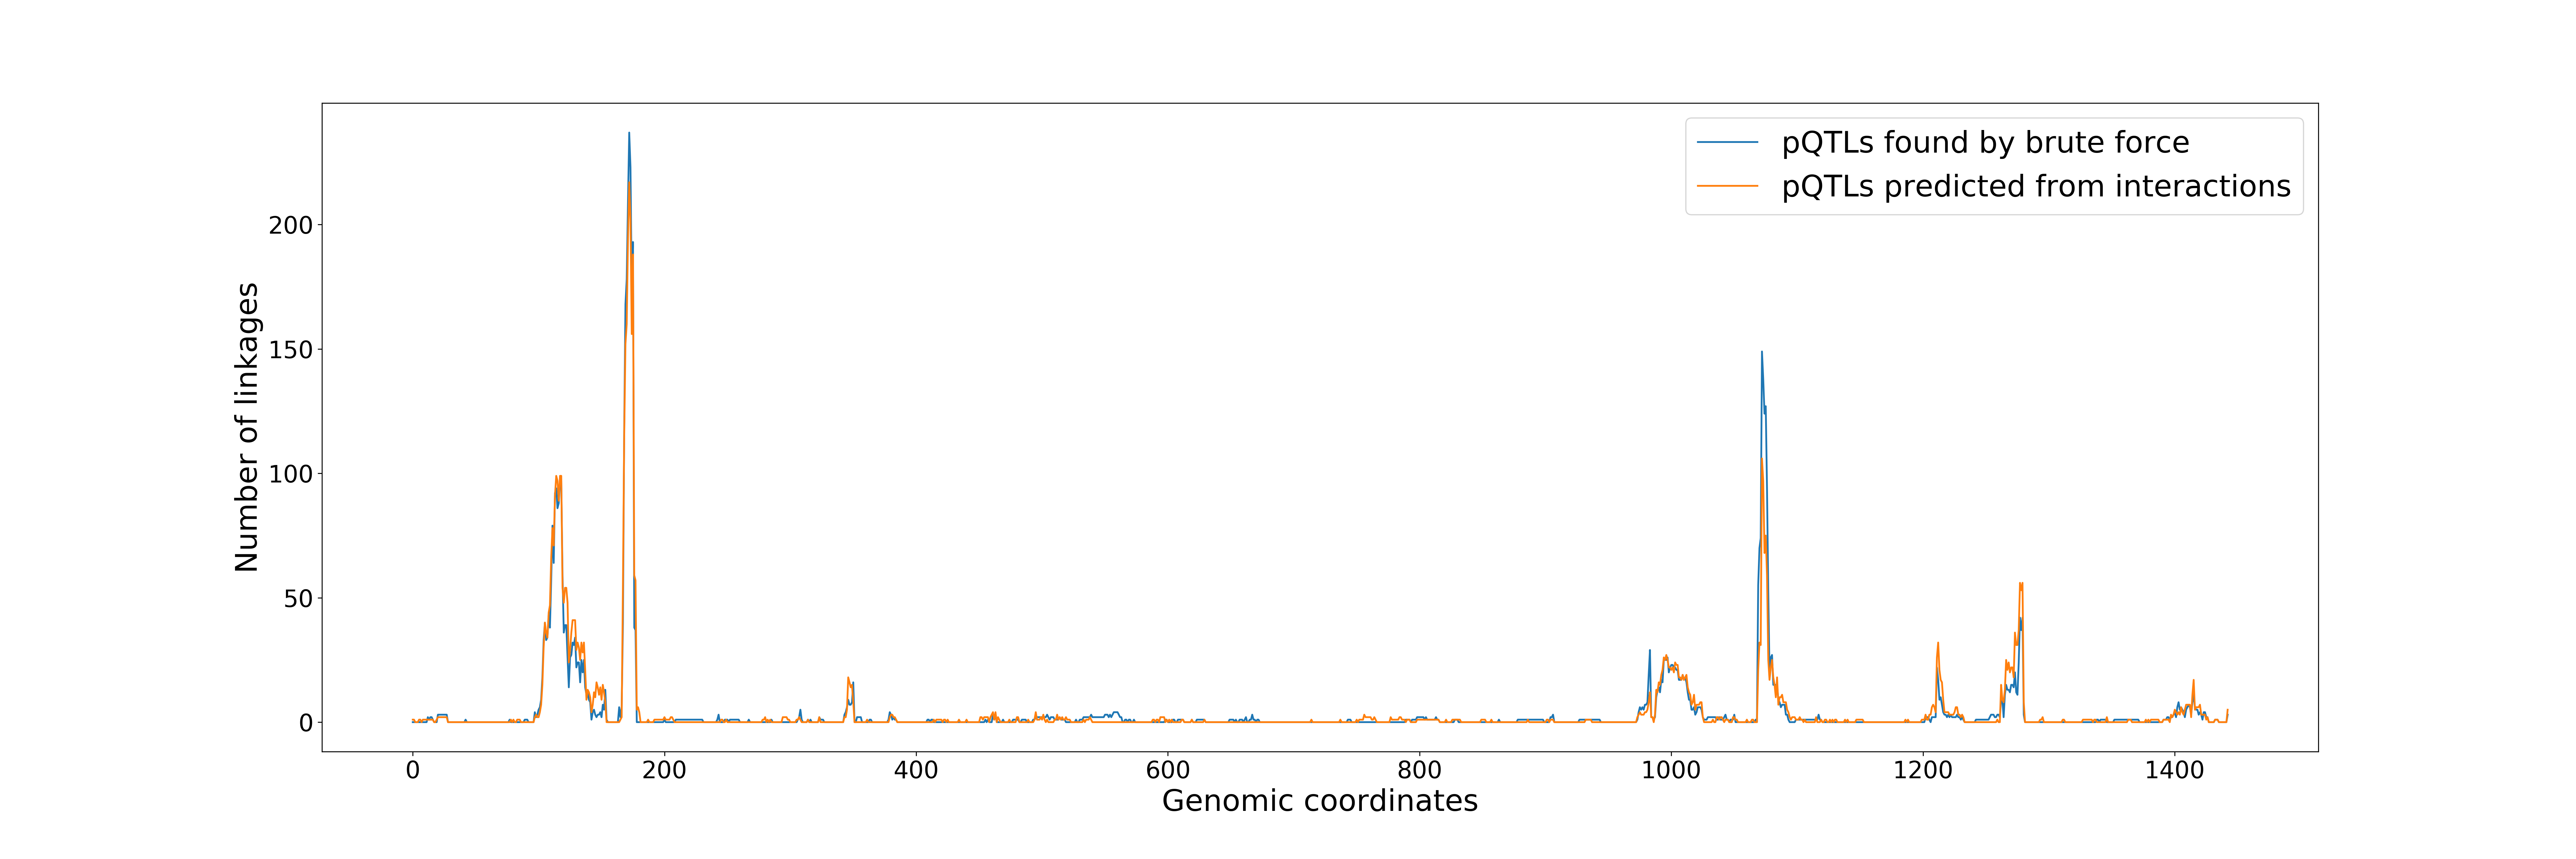
\includegraphics[scale=0.3]{linkages/pQTLs_old_and_new}}
		\end{figure}
		
		Возможность предсказывать достаточно большую долю pQTLs для генов на основе одних только eQTLs для взаимодействующих с ними — аргумент в пользу того, что экспрессия РНК и белковая экспрессия связаны на более глубоком уровне, чем может показаться на первый взгляд. Тем не менее, полученные результаты менее достоверны, чем в предыдущих пунктах, поскольку при проведении анализа появились вопросы к исходным данным, окончательных соглашений по которым пока достигнуто не было. Подробнее об этом написано в  "Методах". 
		
	\subsection{Исследование подобия множеств QTLs в функциональных модулях}
	 На основании статьи \href{https://labs.genetics.ucla.edu/kruglyak/home}{"A global genetic interaction network maps a wiring diagram of cellular function} и данных с \href{http://thecellmap.org/?q=null#}{TheCellMap} в полной сети взаимодействий были выделены функциональные модули, отвечающие фундаментальным клеточным процессам. Саму сеть с изображёнными на ней модулями можно увидеть на рисунке 7, взятом из оригинальной статьи.
		\begin{figure}[H]
			\centering
			\caption{Сеть взаимодействий с TheBioGRID с отмеченными на ней функциональными модулями, полученными с помощью алгоритма \href{http://science.sciencemag.org/content/353/6306/aaf1420}{SAFE}. Далее анализируются именно они.\\ 
			\href{http://science.sciencemag.org/content/353/6306/aaf1420}{"A global genetic interaction network maps a wiring diagram of cellular function", 10.1126/science.aaf1420, 2016}. }
			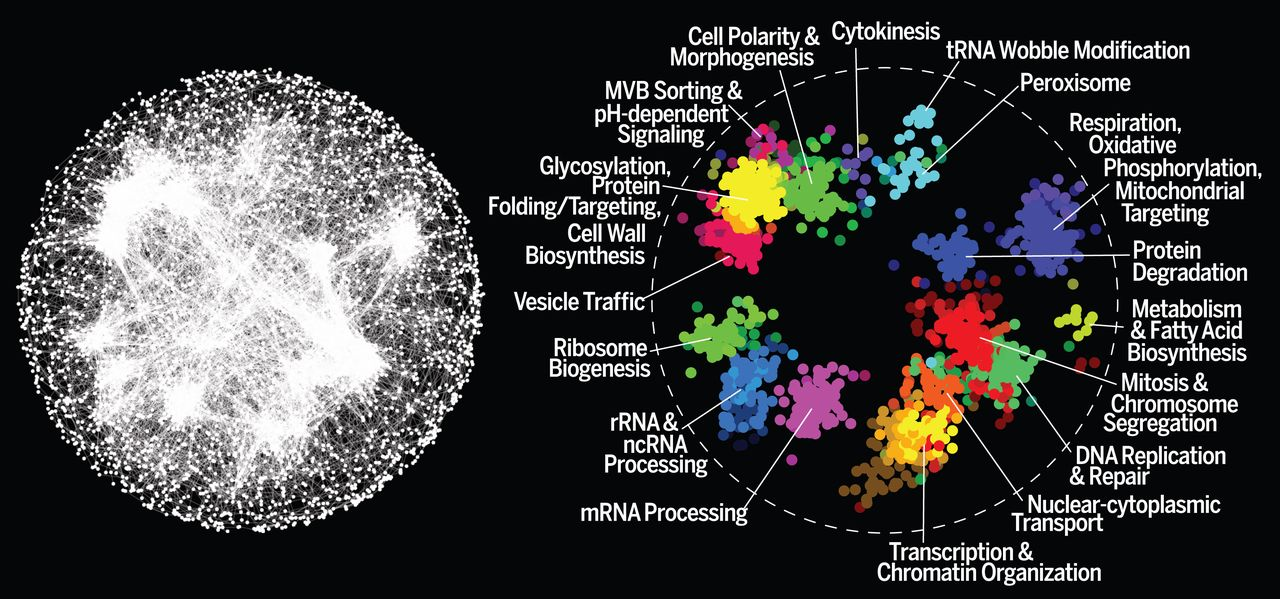
\includegraphics[scale=1.5]{illustrations/Baryshnikova_Functional_Modules.jpg}
		\end{figure}
		Впоследствии были рассмотрены все модули, и для каждого из них был проведен такой же анализ, как во втором и третьем пунктах. То, что получилось, записано в последних трёх столбцах. Для краткости, результаты представлены в виде таблицы, где $\overline{J}_{\text{eQTLs}}(G')$ — среднее значение коэффициента Жаккара для множеств eQTLs взаимодействующих генов, $\overline{J}_{\text{pQTLs}} (G') $ — аналогично для pQTLs. Слева от символа '/' в таблице указано значение для исходного подграфа, справа — значение после рандомизации. Пропуски в последнем столбце — артефакт, обычно появляющийся из-за сочетания малого размера модулей и малого объёма данных, по которым получены pQTLs (в результате для большей части графа взаимодействий они не найдены).:\\
	\begin{tabular} {| L{6cm} | c | c | c | c | C{3cm}| }
		\hline
		\textbf{Название модуля}, порождающего подграф $G' = (V', E')$ & $|V'|$ & $|E'|$ & $\overline{J}_{\text{eQTLs}}(G')$ & $\overline{J}_{\text{pQTLs}} (G')$ & Воспроизведенные pQTLs, \% \\
		\hline 
		Cell polarity \& morphogenesis & 64 & 3118 & 0.154 / 0.135 & 0.117 / 0.216& 67.4 (29/43)\\
		\hline 
		Respiration, oxidative phosphorylation, mitochondrial targeting & 133 & 1206 & 0.185 / 0.075 & 0.487 / 0.41 & 99.1 (107/108)\\
		\hline 
		Protein degradation/turnover & 44 & 2471 & 0.113 / 0.146 & 0.435 / 0.285& 66.7 (2/3)\\
		\hline 
		Ribosome biogenesis & 67 & 251 & 0.269  / 0.36 & 0.198 / 0.193& 87.73 (143/163)\\
		\hline 
		Cytokinesis & 4 & 158 & 0 / 0 & 0 / 0& NA\\
		\hline 
		DNA replication \& repair & 75 & 3605 & 0.073 / 0.055 & 0.346 / 0.196& 75 (66/88)\\
		\hline 
		Nuclear-cytoplasmic transport & 35 & 1134 & 0.082 / 0.111 & 0.622 / 0.481& 72.3 (27/37)\\
		\hline 
		Peroxisome & 17 & 354 & 0.315 / 0.222 & 0 / 0 & NA\\
		\hline 
		Metabolism & 11 & 39 & 0.0 / 0.667 & 0.0 / 0.0& NA\\
		\hline 
		Mitosis \& chromosome segregation & 149 & 11576 & 0.056 / 0.038 & 0.27 / 0.133& 57.64 (49/85)\\
		\hline 
		mRNA \& tRNA processing & 83 & 3437 & 0.073 / 0.107 & 0.592 / 0.021& 61.53 (40/65)\\
		\hline 
		Glycosylation, protein folding/targeting, cell wall biosynthesis & 140 & 8640 & 0.049 / 0.043 & 0.263 / 0.192& 76.12 (118/155)\\
		\hline 
		tRNA wobble modification & 14 & 413 & 0.177 / 0.249 & 0 / 0& NA\\
		\hline 
		rDNA \& ncDNA processing & 76 & 2107 & 0.298 / 0.227 & 0.353 / 0.255& 69.6 (78/112)\\
		\hline 
		Vesicle traffic & 85 & 6108 & 0.114 / 0.081 & 0.342 / 0.194& 30.7 (4/13)\\
		\hline 
		MVB sorting and pH depending signaling & 21 & 353 & 0.174 / 0.446 & 0.4 / 0.556 & NA\\
		\hline 
		Transcription \& chromatin organization & 85 & 6054 & 0.094 / 0.089 & 0.857 / 0.5 & NA\\
		\hline
	\end{tabular}
	\medskip
	
	На основе приведенной таблицы можно сделать вывод, что у взаимодействующих генов в составе одного функционального модуля множества QTLs похожи в среднем больше, чем при рассмотрении случайных подграфрв того же размера. Более того, существенный процент известных pQTLs для таких генов можно предсказать на основе eQTLs соседних с ними генов. Стоит отметить, что их процент гораздо выше, чем при рассмотрении всей сети взаимодействий, как это было сделано в пункте 3. Тем не менее, на этом шаге возникает много вопросов, по которым всё ещё не достигнуты окончательные соглашения. В частности, неясно, что на самом деле считать функциональным модулем, которые из них рассматривать, на каком уровне абстракции о них говорить (а доступный уровень детализации очень высок, вплоть до ансамблей белков, участвующих в реализации какого-то маленького шага клеточного процесса). Также предстоит провести ещё не одну проверку для того, что та взаимосвязь, которая позволяет предсказывать pQTLs по eQTLs, действительно имеет место, а не является артефактом набора данных, выбора функциональных модулей или ещё чего-то. Резюмируя, можно сказать, что к полученным результатам нужно относиться с известной долей осторожности, но тем не менее они достаточно интересные, чтобы проводить дальнейшие исследования.
	
	\section{Выводы}
	
	Во введении была предложена гипотеза: наборы генетических маркеров, управляющих экспрессией РНК — eQTLs — и маркеров, влияющих на белковую экспрессию — pQTLs — согласованы друг с другом на уровне функциональных модулей, несмотря на то, что для отдельных генов статистически значимой взаимосвязи нет. Было решено рассмотреть экспрессию в контексте клеточных процессов, для чего использовались сети белок-белковых взаимодействий. В ходе их совместного анализа было обнаружено, что экспрессия взаимодействующих генов чаще управляется одними и теми же маркерами, чем при рассмотрении случайных пар генов. Более того, было показано, что существует более тонкая взаимосвязь между eQTLs и pQTLs, проявившаяся при рассмотрении сетей: подтвердилось, в целом, разумное предположение, что гены, управляющие экспрессией РНК генов-соседей данного в графе белок-белковых взаимодействий, регулируют и его белковую экспрессию. Оба этих наблюдения оказались более выраженными для функциональных модулей — подграфов сети взаимодействий, соответствующих важным клеточным процессам. Несмотря на то, что многие допущения всё ещё требуют проверки, а результаты ­— биологической интерпретации, есть основания полагать, что гипотеза верна. На основании этого наблюдения планируется далее сформулировать и исследовать понятие module-eQTLs — маркеров, управляющих в некотором смысле экспрессией составляющих функционального модуля как единого целого. При таком подходе, учитывающем не только количественные показатели экспрессии, но и контекст, в котором она происходит, в перспективе поможет лучше понять механизмы протекания клеточных процессов.
	
	\section{Методы:}
	\subsection{Описание данных}
	Провести анализ данных, полученных в 2011 г. исследователями из \href{https://labs.genetics.ucla.edu/kruglyak/home}{Kruglyak lab}. Данные белковой экспрессии были обработаны \href{https://scholar.google.com/citations?user=gJkhFkgAAAAJ&hl=en}{Zia Khan} на основе разработанного им алгоритма. Данные, не находящиеся в открытом доступе, были предоставлены Ю.Л. Притыкиным.\\ 
	\textbf{Краткое описание:} 
	\begin{itemize}
			\item Результаты генотипирования штаммов BY4716 и RM11-1a и 107 штаммов-потомков по набору из 1458 маркеров (наследуемых целиком участков генома, на которых родительские штаммы различны). 
			\item Уровень экспрессии 5610 генов (\href{http://www.thermofisher.com/sg/en/home/life-science/microarray-analysis/affymetrix.html}{Affymetrix microarrays}).
			\item Уровень трансляции 1300 мРНК (масс-спектрометрия).
			\item Сеть белок-белковых взаимодействий с \href{https://thebiogrid.org/}{TheBioGrid Project}. Математически она представляет собой псевдограф на 6611 вершинах и 681490 рёбрах. По типу взаимодействия в ней выделены подграфы со следующими характеристиками:
			\begin{itemize}
				\item Физические взаимодействия: 6314 вершин, 140163 рёбра.
				\item Генетические взаимодействия: 5938  вершин, 541327 рёбер
			\end{itemize}
			\item Данные о функциональных модулях из статьи \href{http://boonelab.ccbr.utoronto.ca/supplement/costanzo2016/}{"A global genetic interaction network maps a wiring diagram of cellular function"}.
	\end{itemize}
	\subsection{Идентификация QTLs}
	Опишем процедуру идентификации eQTLs (случай pQTLs рассматривается аналогично). 
	\begin{enumerate}
		\item Для каждого экспрессируемого гена $ EG_{i} $ и каждого маркера $ M_{j} $ из входного набора данных рассмотреть разбиение данных экспрессии на две независимые выборки $ E_{0}, E_{1} $ согласно варианту маркера, унаследованного организмом. 
		\item Проверить гипотезу, что $ M_{j} $ — eQTL для $ G_{i} $, используя U-критерий Манна-Уитни (\textit{Mann-Whitney U-test}). Порог p-значений — 0.001.
		\item С помощью алгоритма \href{https://github.com/StoreyLab/qvalue}{q-value} провести FDR-коррекцию множества $ \{ p_{i, j} \} $ полученных p-значений для всех пар $ (G_{i}, M_{j}) $. Допустимая доля $ \alpha $ ошибок первого рода — 0.05.
	\end{enumerate}
	\subsection{Исследование подобия множеств QTLs у взаимодействующих генов}
	Для каждого типа QTLs, для каждого графа взаимодействий $ G_{I} $ и заданного множества $ \{q_{i}\}_{i=0}^{M},\ 0 < q_{1} < q_{2} < \dots < q_{M} = 0.001 $ порогов q-значений провести серию из $ M $ экспериментов. Результатом каждого из них будут два значения: усреднённая мера подобия множеств QTLs каждого типа для взаимодействующих и случайных пар генов.
	\begin{enumerate}
		\item На $ k $-ой итерации убрать из рассмотрения те eQTLs, q-значения которых превышают текущий порог $ q_{k} $. Обозначим множество оставшихся eQTLs для гена $ g $ через $ \mbox{eQTLs}_{k}(g) $.
		\item Сгенерировать последовательность графов $ \{G_{I, n}\}_{n=0}^{N},\  G_{I, 0} := G_{I} $, полученных рандомизацией графа $ G_{I} $ с сохранением определённых инвариантов (набора степеней вершин, распределения степеней вершин и т.д.). 
		\item Вычислить последовательность \[ J_{k, i} := \left (\sum_{(u, v) \in E(G_{I, i})}{\mu_{J}\left (\mbox{eQTLs}_{k}(u), \mbox{eQTLs}_{k}(v)\right )}\right )/\left |E(G_{I, i})\right |\]
		где $ \mu_{J}(A, B) := \frac{|A \cap B|}{|A \cup B|} $ — коэффициент Жаккара.
		\item Вернуть значения $ J_{k,0} $ и $ \left (\sum_{i=1}^{N}{J_{k,i}}\right )/N $.
	\end{enumerate}
	На основе полученных данных построить график, на котором наглядно видно, что мера подобия для исходного графа выше, чем для случайного графа аналогичной структуры.\\
	Для большей строгости, можно на каждой итерации запомнить коэффициент Жаккара для каждого ребра, составить две выборки — для исходного и случайных графов — и проверить для них гипотезу с помощью критерия Манна-Уитни. Пока что этот шаг находится на этапе реализации.\\
	Заметим, что наличие в графе петель и кратных рёбер очевидным образом приводит к инфляции коэффициента Жаккара. Тем не менее, было принято решение их из графа взаимодействий не удалять, т.к. их очень много, они не бессмысленны с точки зрения биологии и не влияют на ответ качественно, только количественно.
	\subsection{Предсказание pQTLs на основе eQTLs}
	\begin{enumerate}
		\item По данному подграфу графа взаимодействий сгенерировать множество пар маркер-ген, где маркер — кандидат в pQTLs для данного гена. В качестве маркеров-кандидатов положить eQTLs вершин-соседей в графе взаимодействий, включая сам исследуемый ген. 
		\item Для полученного множества пар провести тот же анализ, что в пункте 5.2., с тем же пороговым $ q $-значением. 
		\item Сравнить множества получившихся pQTLs с теми, что были вычислены полным перебором.
	\end{enumerate}
	При реализации алгоритма был поднят вопрос о том, что именно считать маркерами, поскольку в исходных данных с генотипами штаммов на большинстве маркеров в смысле их исходного определения (согласованно наследуемая последовательность нуклеотидов, такая что в скрещиваемых штаммах содержатся разные её варианты) были поставлены несколько меток — подпоследовательностей нуклеотидов, которые связывались с субстратом на микрочипе. Таким образом в файле с генотипами одному гену де-факто соответствовали несколько: по одному на каждую метку. Ясно, что такой подход оправдан с точки зрения надёжности результатов эксперимента. Тем не менее, пока что авторы не пришли к окончательному соглашению о том, считать ли метки отдельными маркерами или нет. Проблема в том, что они вызывают инфляцию значения коэффициента Жаккара: де-факто вместо одной связи (маркер-ген) получается много практически неразличимых копий, из-за чего итоговое значение получается больше, чем нужно. Более того, такие дубликаты искажают общую картину хотя бы силу проблемы multiple testing burden: hotspots, с которыми итак связано много генов, подавляют за счёт дубликатов менее выраженные QTLs. Пока что было принято решение дубликаты удалить, а характер наследования определять голосованием. Тем не менее, при таком подходе получается воспроизвести меньше pQTLs, чем ранее удавалось научному руководителю, который дубликаты не удалял. В связи с этим много времени и усилий было потрачено на то, чтобы попытаться воспроизвести старые результаты или понять, почему они не воспроизводятся. Этот вопрос всё ещё требует дополнительного исследования. Стоит отметить, что этот выбор не влияет на результаты с точки зрения распределения QTLs в геноме и положения hotspots в нём, а основной объект исследования в данной работе — именно они.
	\subsection{Исследование подобия множеств QTLs в функциональных модулях}
	На основе аннотации из статьи \href{https://labs.genetics.ucla.edu/kruglyak/home}{"A global genetic interaction network maps a wiring diagram of cellular function} выделить подграфы, отвечающие конкретным клеточным процессам. Провести для них тот же анализ, что в пункте 5.2. Затем провести достаточно много (сотни, тысячи) тестов двух типов: проверить, что получаемые значения выше и чем для случайных подграфов того же размера, и чем для подграфов на тех же вершинах после рандомизации сети взаимодействий с сохранением определённых инвариантов (набора или распределения степеней вершин). Тестирование по первому типу пока не реализовано, но в скором будущем будет.\\
	В ходе обсуждения постановки задачи с научным руководителем было решено, что правильно было бы выделять функциональные модули иначе: следует подняться на определённую высоту в дереве аннотаций на GeneOntology, выбрать все поддеревья, содержащие не менее чем сколько-то вершин и не более чем столько-то вершин и считать модулями уже их. Как минимум, это надёжнее с точки зрения статистики, т.к. выбор кластеров основан не на их содержательном смысле, а на некоторых количественных характеристиках, которые легко варьировать, чтобы проверять, остаётся ли проверяемая гипотеза верна или нет. Тем не менее, это обсуждалось недавно, в связи с чем идея пока что не реализована, а взятые из статьи кластеры было решено оставить для наглядности.
	\subsection{Вычислительный эксперимент}
	Весь написанный код в формате .ipynb-ноутбука находится в открытом доступе. Тем не менее, проект всё ешё в стадии разработки и часто меняется, так что комментарии могут быть неполны.\\ \url{https://github.com/ivanov-v-v/eQTL_analysis}\\
	Графики и данные можно найти там же. В целом, была поставлена задача добиться воспроизводимости полученных результатов. Ознакомиться с интересными примерами такого подхода, использующего возможности Jupyter Notebook как платформы для написания интерактивных документов, можно \href{https://github.com/jupyter/jupyter/wiki/A-gallery-of-interesting-Jupyter-Notebooks#reproducible-academic-publications}{по ссылке}.\\
	Идентификация QTLs реализована двумя способами: на numpy/scipy (в силу больших объёмов данных для проведения анализа таким образом были запрошены вычислительные мощности суперкомпьютерного кластера МФТИ) и с помощью пакета \href{http://www.bios.unc.edu/research/genomic_software/Matrix_eQTL/}{MatrixEQTL} для языка R.\\ 
	FDR-коррекция реализована на R с помощью пакета \href{http://www.bioconductor.org/packages/release/bioc/html/qvalue.html}{qvalue}.\\
	Для работы с графами в Python была использована библиотека \href{http://igraph.org/redirect.html}{igraph}.
	
	\begin{thebibliography}{}
		\bibitem{GTEx2017} GTEx Consortium — "Genetic effects on gene expression across human tissues" — doi:10.1038/nature24277
		\bibitem{Huttlin-2017} Edward L. Huttlin, Raphael J. Bruckner et al — "Architecture of the human interactome defines
		protein communities and disease networks" — doi:10.1038/nature22366
		\bibitem{Kruglyak2002} Rachel B. Brem, Gaël Yvert, Rebecca Clinton, Leonid Kruglyak — "Genetic Dissection of Transcriptional Regulation in Budding Yeast" — doi: 10.1126/science.1069516
		\bibitem{Kruglyak2005} Rachel B. Brem, Leonid Kruglyak — "The landscape of genetic complexity across 5,700 gene expression traits in yeast" — doi: 10.1073/pnas.0408709102 
		\bibitem{Kruglyak2015} Frank W. Albert, Leonid Kruglyak — "The role of regulatory variation in
		complex traits and disease" — doi:10.1038/nrg3891
		\bibitem{Kruglayk2017} Frank W. Albert, Joshua S. Bloom, Jake Siegel, Laura Day, Leonid Kruglyak — "Genetics of trans-regulatory variation in gene expression" — https://doi.org/10.1101/208447
		\bibitem{Fortunato} Santo Fortunato — "Community detection in graphs" — arXiv:0906.0612v2
		\bibitem{Ideker-Nussinov-2017} Trey Ideker, Ruth Nussinov — "Network approaches and applications in biology" — doi.org/10.1371/journal.pcbi.1005771
		\bibitem{Costanzo2009} Michael Costanzo, Anastasia Baryshnikova et al. — "The Genetic Landscape of a Cell" — doi: 10.1126/science.1180823
		\bibitem{Costanzo2016} Michael Costanzo, Benjamin VanderSluis, Elizabeth N. Koch, Anastasia Baryshnikova et al. — "A global genetic interaction network maps a wiring diagram of cellular function"
	\end{thebibliography}
\end{document}